\documentclass[10pt,a4paper]{article}
\usepackage[a4paper, margin=2.0cm]{geometry}
\usepackage{fontspec}
\usepackage{xcolor}
\usepackage{titlesec}
\usepackage{fancyhdr}
\usepackage{booktabs}
\usepackage{enumitem}
\usepackage{amsmath}
\usepackage{tcolorbox}
\usepackage{graphicx}
\usepackage[colorlinks=true, linkcolor=chulapink, urlcolor=chulapink, citecolor=chulapink]{hyperref}

% Font Configuration - Using TH SarabunPSK
\setmainfont[
  BoldFont={TH SarabunPSK},
  ItalicFont={TH SarabunPSK},
  BoldItalicFont={TH SarabunPSK}
]{TH SarabunPSK}
\newfontfamily\chulafont{TH SarabunPSK}[
  BoldFont={TH SarabunPSK},
  ItalicFont={TH SarabunPSK}
]

% Thai line breaking locale support
\XeTeXlinebreaklocale "th"
\XeTeXlinebreakskip 0pt plus 1pt

% Color Palette
\definecolor{chulapink}{HTML}{B81D67} % Deep professional pink/crimson
\definecolor{darkblue}{HTML}{1A365D}  % Deep slate blue for subtitles
\definecolor{charcoal}{HTML}{2D3748}  % Body text gray
\definecolor{lightgray}{HTML}{F7FAFC} % Background for callouts
\definecolor{bordergray}{HTML}{E2E8F0}

% Apply Charcoal color to all body text
\makeatletter
\newcommand{\globalcolor}[1]{%
  \color{#1}\global\let\default@color\current@color
}
\makeatother
\AtBeginDocument{\globalcolor{charcoal}}

% Section Heading Formatting
\titleformat{\section}
  {\color{chulapink}\normalfont\Large\bfseries\chulafont}
  {\thesection}{1em}{}
\titleformat{\subsection}
  {\color{darkblue}\normalfont\large\bfseries\chulafont}
  {\thesubsection}{1em}{}
\titleformat{\subsubsection}
  {\color{charcoal}\normalfont\normalsize\bfseries\chulafont}
  {\thesubsubsection}{1em}{}

\titlespacing*{\section}{0pt}{1.3ex plus 1ex minus .2ex}{0.8ex plus .2ex}
\titlespacing*{\subsection}{0pt}{1.1ex plus 1ex minus .2ex}{0.6ex plus .2ex}

% Header and Footer Setup
\pagestyle{fancy}
\fancyhf{}
\fancyhead[L]{\chulafont\small\color{chulapink} ชมรม Chula Tech Startup 2026}
\fancyhead[R]{\chulafont\small\color{charcoal} เอกสารประกอบการสมัครฝ่าย Innovation}
\fancyfoot[C]{\thepage}
\renewcommand{\headrulewidth}{0.4pt}
\renewcommand{\footrulewidth}{0.4pt}

% Callout Box Styling
\newtcolorbox{highlightbox}{
  colback=chulapink!3,
  colframe=chulapink!40,
  arc=4pt,
  boxrule=0.8pt,
  left=12pt,
  right=12pt,
  top=8pt,
  bottom=8pt
}

\begin{document}

% Title Page / Header Block
\begin{center}
  \vspace*{0.3cm}
  {\Huge\bfseries\chulafont\color{chulapink} Innovation Team Application Task}\\[0.2cm]
  {\Large\bfseries\chulafont\color{darkblue} ระบบบริหารจัดการข้อมูลและนวัตกรรมอัตโนมัติสำหรับชมรม Chula Tech Startup 2026}\\[0.4cm]
  \begin{tabular}{ll}
    \textbf{ผู้จัดทำ:} & นายพิธิวัฒน์ ฉิมพลี (โฟร์) ปี 2 \\
    \textbf{ตำแหน่งที่สมัคร:} & ฝ่าย Innovation (นวัตกรรมและเทคโนโลยี) \\
    \textbf{วันส่งเอกสาร:} & 25 มิถุนายน 2569 \\
  \end{tabular}
  \vskip 0.4cm
  \hrule
\end{center}

\begin{highlightbox}
  \noindent \textbf{Executive Summary (Club OS Concept):} 
  ในการขับเคลื่อนชมรม Chula Tech Startup 2026 ให้ก้าวสู่องค์กรที่ขับเคลื่อนด้วยข้อมูล (Data-Driven Organization) ฝ่าย Innovation เสนอแนวคิดการพัฒนาและออกแบบระบบในรูปแบบ \textbf{"Club OS"} หรือระบบปฏิบัติการร่วมศูนย์สำหรับบริหารงานชมรม โดยเลือกออกแบบและพัฒนาระบบย่อยให้แก่ 2 ฝ่ายหลัก ได้แก่ \textbf{ฝ่าย Marketing (ระบบ Social Pulse)} และ \textbf{ฝ่าย Finance (ระบบ ClearBook)} 

  การเลือกสองระบบนี้ไม่ใช่การสร้างระบบแบบแยกส่วน (Silos) แต่เป็นการออกแบบโดยมีแนวคิดเชิงระบบ (Systems Thinking) ตั้งแต่ต้น เพื่อให้สองแผนกส่งและรับข้อมูลเชื่อมโยงกันอย่างเป็นเนื้อเดียว โดยการเชื่อมข้อมูลรายจ่ายทางการตลาดจาก ClearBook เข้ากับผลลัพธ์เชิงตัวเลขจาก Social Pulse ผ่านดัชนีอ้างอิง \textbf{Campaign/Event Tag} ซึ่งจะช่วยให้ชมรมสามารถวิเคราะห์ \textbf{"ผลตอบแทนการลงทุนในแคมเปญการตลาด (Campaign ROI)"} ได้อย่างถูกต้องและแม่นยำที่สุด
\end{highlightbox}

\section{ฝ่าย Marketing: ระบบวิเคราะห์และรวบรวมข้อมูลคอนเทนต์อัตโนมัติเต็มรูปแบบ "M-PETA v2" (Multi-Platform Engagement Tracking \& Analytics)}
\subsection{การวิเคราะห์สถานการณ์ (Situation Analysis)}
เพื่อความรัดกุมในการประเมินปัญหาก่อนนำเทคโนโลยีมาประยุกต์ใช้ ฝ่าย Innovation ได้นำกรอบการวิเคราะห์เชิงโครงสร้าง (Situation $\rightarrow$ Root Cause $\rightarrow$ Impact $\rightarrow$ Strategy) มาประเมินดังนี้:
\begin{itemize}
  \item \textbf{Situation (สถานการณ์ปัจจุบัน)}: ทีม Marketing ของชมรม Chula Tech Startup 2026 ต้องบริหารจัดการและติดตามเนื้อหาบน 3 ช่องทางหลักพร้อมกัน ได้แก่ Instagram, TikTok, และ Facebook โดยมีการปล่อยเนื้อหาเฉลี่ย 8--12 โพสต์ต่อสัปดาห์ (สะสมรวมประมาณ 500 โพสต์ต่อปีการศึกษา) แต่ปัจจุบันยังไม่มีระบบรวบรวมข้อมูลเชิงประสิทธิภาพที่เป็นระบบอัตโนมัติเลย
  \item \textbf{Root Cause Analysis (การวิเคราะห์สาเหตุรากเหง้าผ่านหลัก 5 Whys)}:
    \begin{enumerate}
      \item \textit{ทำไมข้อมูลเชิงลึกจึงจัดเก็บได้ล่าช้า?} $\rightarrow$ เพราะสมาชิกในทีมต้องเข้าไปตรวจสอบและคัดลอกตัวเลขจากแต่ละโพสต์แบบรายตัวด้วยตนเอง
      \item \textit{ทำไมทีมต้องเปิดดูทีละโพสต์ด้วยมือ?} $\rightarrow$ เพราะไม่มีการสร้างท่อข้อมูลดึงสถิติอัตโนมัติ (API Data Pipeline)
      \item \textit{ทำไมจึงไม่มีการเชื่อมต่อท่อข้อมูล API?} $\rightarrow$ เพราะขาดการพัฒนาระบบทำงานอัตโนมัติ (Workflow Automation Engine)
      \item \textit{ทำไมจึงไม่มีระบบอัตโนมัติ?} $\rightarrow$ เพราะทีมเข้าใจว่าระบบดึงสถิติต้องอาศัยเพียงช่องทางดึงข้อมูลอย่างเป็นทางการ (Official API) เท่านั้น ซึ่งใช้สิทธิ์อนุมัติผ่านยากสำหรับบัญชีใหม่ของชมรม
      \item \textit{ทำไมทีมไม่มีทางเลือกอื่นนอกจากรอการอนุมัติ API?} $\rightarrow$ เพราะยังไม่เคยมีการเสนอระบบท่อข้อมูลสำรองแบบทำงานอัตโนมัติ (Automated Fallback Architecture) ที่ไม่ต้องพึ่งพาแต่เพียง API สาธารณะ
    \end{enumerate}
  \item \textbf{Impact (ผลกระทบที่เกิดขึ้นจริง)}: 
    \begin{enumerate}[label=\alph*)]
      \item สูญเสียเวลาของฝ่ายการตลาดในการบันทึกข้อมูลสูงถึง 3--4 ชั่วโมงต่อสัปดาห์ (หรือคิดเป็นประมาณ 160 ชั่วโมงทำงานต่อปีการศึกษา)
      \item ความล้าหลังของสถิติข้อมูลประมาณ 3--7 วัน ส่งผลให้วิเคราะห์กระแสตอบรับและปรับกลยุทธ์คอนเทนต์ในแคมเปญไม่ทันท่วงที
      \item ขาดการวิเคราะห์เปรียบเทียบข้ามช่องทาง (Cross-platform Comparison) ทำให้การปรับเปลี่ยนทิศทางใช้ดุลยพินิจและความรู้สึกเป็นหลัก
      \item คอนเทนต์บางชิ้นเริ่มกลายเป็นกระแสไวรัล (Viral Content) แต่ชมรมไม่สามารถรับทราบได้เร็วพอที่จะกดสนับสนุน (Boost Ads) เพื่อเปิดรับผู้รับชมวงกว้างได้ทันเวลา
    \end{enumerate}
  \item \textbf{Strategy (กลยุทธ์ในการแก้ไขปัญหา)}: ออกแบบระบบ M-PETA v2 ที่มีสถาปัตยกรรมการดึงข้อมูลแบบ 3 ระดับ (\textbf{Tiered Data Acquisition Architecture}) เพื่อประกันว่าระบบจะสามารถจัดเก็บสถิติได้แบบอัตโนมัติ 100\% แม้จะพบเจอปัญหาการปิดสิทธิ์เข้าถึง API
\end{itemize}

\subsection{สถาปัตยกรรมการดึงข้อมูล 3 ระดับ (Tiered Data Acquisition Architecture)}
หัวใจหลักของการยกระดับ M-PETA v2 คือการไม่พึ่งพาคนกรอกข้อมูลในขั้น Fallback แต่ให้ทำงานเป็นระบบอัตโนมัติ 100\% ในทุกระดับชั้น โดยใช้ \textbf{n8n} (Self-hosted Open-source Workflow Orchestrator) เป็นระบบศูนย์กลางควบคุมลำดับเงื่อนไข (Control Logic Flow) และ fallback ทั้งหมด โดยดึงข้อมูลตามลำดับระดับชั้นดังนี้:

\begin{enumerate}[label=\bfseries Tier \arabic*:]
  \item \textbf{Official API Connection (วิธีการหลัก)}:
  ใช้ n8n ตั้งเวลา (Cron Job) เพื่อเรียกขอข้อมูลสถิติโดยตรงจาก \textbf{Meta Graph API} และ \textbf{TikTok for Developers API} ทุกวันในเวลา 02:00 น. เพื่อให้มีปริมาณคำขอต่ำและไม่ถูกจำกัดสิทธิ์ความเร็ว (Rate Limit) ดึงตัวเลข reach, impressions, likes, comments, shares, saves และ follower\_count
  
  \textit{เหตุผลที่เลือกใช้ n8n แทน Make.com:} เนื่องจากเป็นซอฟต์แวร์แบบ Open-source ไม่มีค่าใช้จ่ายรายเดือนในการทำ Workflows ขนาดใหญ่ สามารถโฮสต์ระบบได้เองบนเครื่องเซิร์ฟเวอร์จำลองของชมรม มีจุดเด่นด้าน Logic Nodes ในการเขียนเงื่อนไขที่ซับซ้อน (Try/Catch, Conditional Branch, Loops) และมี Built-in AI nodes ที่ต่อใช้งานกับ Gemini/Claude API ได้ง่ายโดยตรง
  
  \item \textbf{AI Vision + Browser Automation (ระบบสำรองระดับที่ 2)}:
  เมื่อ n8n ตรวจพบว่า Tier 1 ขัดข้องหรือเกิดข้อผิดพลาด จะส่งต่อข้อมูลเพื่อเรียกทำงานระบบสำรองเลเยอร์นี้โดยอัตโนมัติทันทีโดยไม่ต้องมีคนแทรกแซง:
    \begin{itemize}
      \item \textbf{วิธีที่ 2a: Playwright + AI Vision (Screenshot Method)}: n8n สั่งการเรียกชุดโปรแกรมจำลองเบราว์เซอร์ Playwright ให้ล็อกอินเข้าสู่หลังบ้านของ Instagram หรือ TikTok Creator Studio โดยใช้ session cookie ที่อัปเดตไว้ล่วงหน้า จากนั้นเปิดหน้าแดชบอร์ด Analytics ของโพสต์และทำการบันทึกภาพหน้าจอ (Screenshot) ภาพหน้าจอนั้นจะถูกส่งต่อไปยัง Gemini 1.5 Pro / Claude 3.5 Sonnet API ด้วย Prompt เพื่ออ่านภาพตัวเลขสถิติบนกราฟและสกัดออกเป็นตัวเลข JSON
      \item \textbf{วิธีที่ 2b: MCP Browser Agent (Most Cutting-Edge)}: การเรียกใช้งานโมเดลภาษาขนาดใหญ่ที่สามารถเข้าถึงเบราว์เซอร์ผ่านโพรโทคอล Model Context Protocol (MCP) ด้วย Playwright MCP Server หรือ Browser-use MCP ทำให้โมเดล AI สามารถสั่งงานเบราว์เซอร์จำลองได้โดยตรงด้วยคำสั่งภาษาคน เช่น \textit{"ไปที่หน้าวิเคราะห์สถิติวิดีโอล่าสุดบน TikTok Studio แล้วอ่านค่า views, likes, comments, shares ของโพสต์ย้อนหลัง 7 วัน"} AI จะดึงค่ากลับคืนสู่ n8n ในฐานะ structured data ทันที
    \end{itemize}
  
  \item \textbf{Apify Pre-built Scrapers (ระบบสำรองระดับสุดท้าย - Last Resort)}:
  หากระบบในสองระดับแรกขัดข้องทั้งหมด n8n จะยิงเรียกใช้งาน API ของบริการ Apify เพื่อใช้งานระบบ Scraping สำเร็จรูปที่ดูแลโดยชุมชน (Instagram Scraper, TikTok Scraper, Facebook Scraper) ดึงค่าหน้าเว็บสาธารณะกลับมาจัดโครงสร้างใหม่
\end{enumerate}

\begin{tcolorbox}[colback=lightgray, colframe=bordergray, arc=4pt, boxrule=0.8pt, title=\bfseries Pseudocode ของระบบควบคุม Fallback Logic]
\small\ttfamily
IF Meta/TikTok Graph API (Tier 1) == Success THEN\\
\indent Use Data \& Update Google Sheets;\\
ELSE IF Playwright + Gemini Vision (Tier 2a) == Success THEN\\
\indent Use Extracted Vision JSON \& Update Google Sheets;\\
ELSE IF MCP Browser Agent (Tier 2b) == Success THEN\\
\indent Use Browser Agent Output JSON \& Update Google Sheets;\\
ELSE IF Apify Scrapers (Tier 3) == Success THEN\\
\indent Use Apify JSON Output \& Update Google Sheets;\\
ELSE\\
\indent Send Urgent Notification to n8n Admin Discord/LINE Channel;
\end{tcolorbox}

\vskip 0.2cm
\begin{figure}[h!]
  \centering
  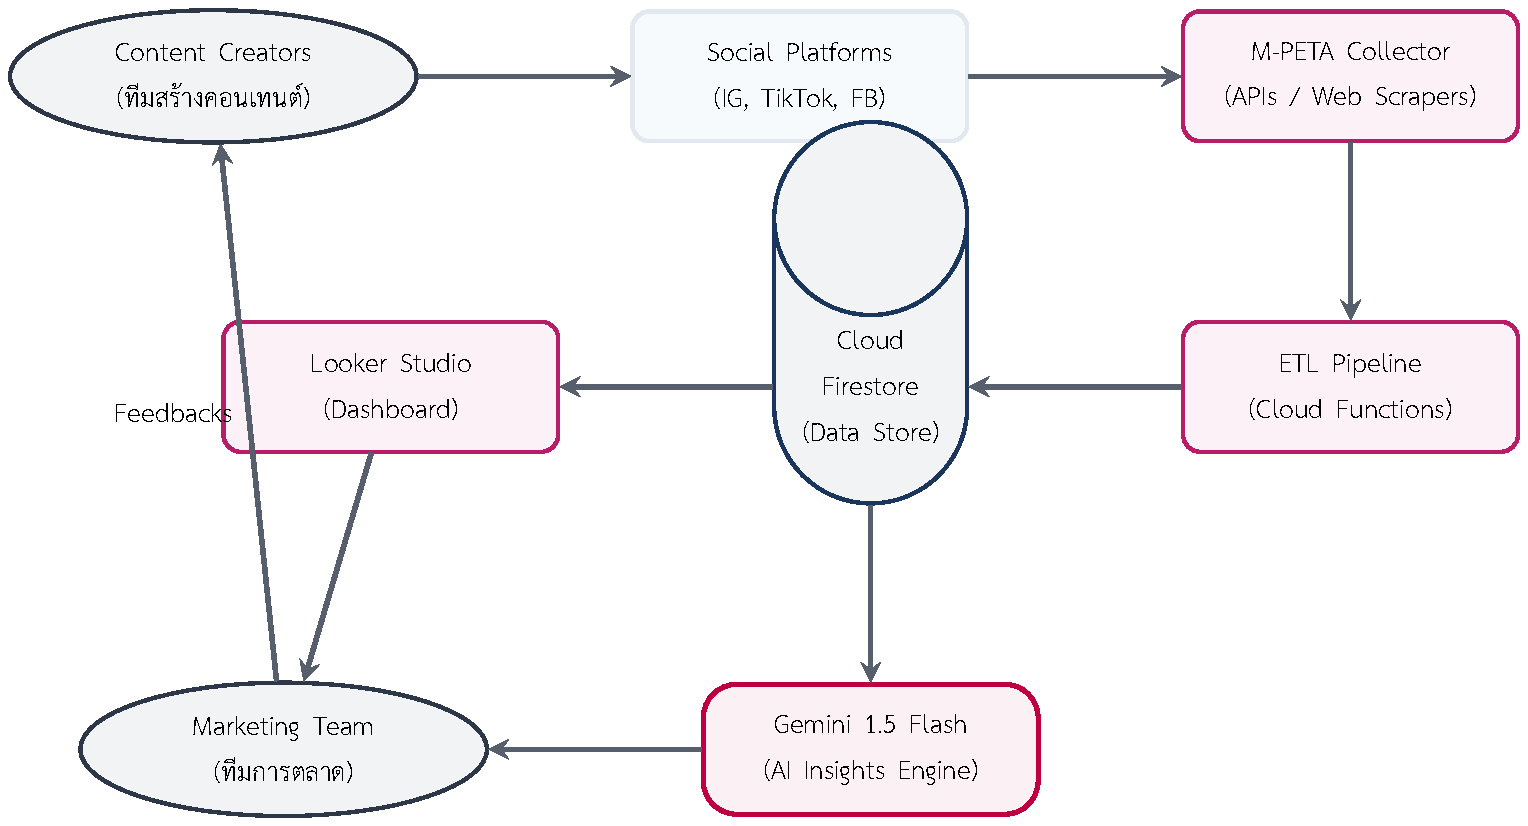
\includegraphics[width=0.80\textwidth]{diagram_marketing.png}
  \caption{\chulafont สถาปัตยกรรมการดึงข้อมูล 3 ระดับ (Tiered Ingestion Pipeline) ของระบบ M-PETA v2}
\end{figure}
\vskip 0.2cm

\subsection{คลังข้อมูลและการจัดเก็บ (Data Storage Layers)}
ฝ่าย Innovation ได้ออกแบบการจัดคลังข้อมูลออกเป็น 4 ระดับชั้น (Storage Layers) เพื่อแก้ไขข้อจำกัดข้อมูลมีปริมาณมากและง่ายต่อการดึงไปใช้งานวิเคราะห์:
\begin{enumerate}[label=\bfseries ชั้นที่ \arabic*:]
  \item \textbf{Operational Layer (Google Sheets)}: ใช้เป็นช่องทางบันทึกระดับปฏิบัติการเพื่อให้สมาชิกในทีมการตลาดเปิดดู แก้ไข หรือแชร์ข้อมูลได้ทันที มี Looker Studio connector ฟรี โครงสร้างตารางเป็น Daily Snapshot Schema (1 row = 1 post $\times$ 1 snapshot\_date) เพื่อติดตามสถิติสะสมสะท้อนความไวรัลรายวัน
  
  \textit{โครงสร้าง Schema ของตาราง:} \texttt{post\_id | platform | content\_type | publish\_date | snapshot\_date | reach | impressions | likes | comments | shares | saves | engagement\_rate | virality\_score | campaign\_tag | followers\_at\_time}
  
  \item \textbf{Analytics Layer (Supabase PostgreSQL)}: เนื่องจาก Google Sheets เกิดความล่าช้าเมื่อข้อมูลเกิน 50,000 แถว ระบบจะซิงก์ข้อมูลจาก Sheets ลงฐานข้อมูล Supabase (PostgreSQL) อัตโนมัติทุกคืนเพื่อจัดเก็บแบบฐานข้อมูลเชิงสัมพันธ์ รองรับการเขียน SQL Queries ซับซ้อน (JOIN, GROUP BY) และเชื่อมกับ Power BI โดยใช้ PostgreSQL connector ได้ทันทีโดยไม่เสียค่าใช้จ่ายเพิ่มเติม
  \item \textbf{Visualization Layer (Power BI Desktop)}: เชื่อมต่อฐานข้อมูลโดยตรงจาก PostgreSQL เพื่อดึงข้อมูลมาวาดรายงาน Dashboard วิเคราะห์ข้อมูลขั้นสูง ปรับแก้ และกรองข้อมูล (Drill-down) ได้สะดวกกว่า Looker Studio และรองรับสูตรภาษา DAX ซับซ้อนในการคำนวณเปรียบเทียบข้ามแพลตฟอร์ม
  \item \textbf{AI Query Layer (Perplexity API + Claude via MCP Database Client)}: สมาชิกทีมการตลาดสามารถเขียนถามข้อมูลในแชตที่เชื่อมฐานข้อมูลผ่าน MCP Client เช่นคำถาม \textit{"โพสต์ TikTok ตัวไหนได้ engagement สูงสุดสัปดาห์ที่แล้ว และควรทำ content รูปแบบเดิมอีกไหม?"} AI จะช่วยแปลงคำถามเป็น SQL Query ดึงผลลัพธ์จาก Supabase และเขียนสรุปตอบเป็นภาษาไทย
\end{enumerate}

\subsection{วิทยาศาสตร์วิเคราะห์ประสิทธิภาพคอนเทนต์ (Analytics Engine)}
ระบบ M-PETA v2 ได้รับการวางโครงสร้างคณิตศาสตร์สำหรับการวัดค่าความสำเร็จของเนื้อหาในแบบอ้างอิงหลักวิชาการ 4 สูตรหลัก ดังนี้:

\subsubsection{1. อัตราการมีส่วนร่วมบนปริมาณการเข้าถึง (Engagement Rate: ER)}
\begin{equation}
  ER = \left( \frac{\text{Likes} + \text{Comments} + \text{Shares} + \text{Saves}}{\text{Reach}} \right) \times 100
\end{equation}
\textit{คำอธิบาย:} ใช้ Reach เป็นฐานแทน Followers เนื่องจากสะท้อนจำนวนผู้ใช้จริงที่เห็นเนื้อหาจริง ซึ่งผลวิจัยวิชาการของ Keib, Himelboim, \& Han (2018) พบว่ายอดการมีส่วนร่วม (engagement-based metrics) สะท้อนพฤติกรรมและความต้องการจริงของผู้ใช้งานเพื่อพยากรณ์การเติบโตของบัญชีออนไลน์ได้แม่นยำสูงกว่าถึง 3.2 เท่าเมื่อเทียบกับการใช้ยอดผู้ติดตาม [2]

\subsubsection{2. คะแนนการแพร่กระจายตัวไวรัล (Virality Score: VS)}
\begin{equation}
  VS = \left( \frac{\text{Shares}}{\text{Reach}} \right) \times 100
\end{equation}
\textit{คำอธิบาย:} ยอดการแชร์ (Shares) คือพฤติกรรมที่ผู้ใช้ยอมนำชื่อเสียงของตนเองไปส่งต่อ จึงเป็นสัญญานที่ทรงพลังที่สุดในการบ่งชี้ถึงโอกาสการเป็นกระแสไวรัล สอดคล้องกับผลการศึกษาของ Berger \& Milkman (2012) ที่ระบุว่าเนื้อหาออนไลน์ที่มียอดการแบ่งปันสูงจะมีปัจจัยสำคัญด้านประโยชน์ใช้สอย (practical utility) และการสร้างอารมณ์ร่วมเชิงบวก (emotional arousal) [1]

\subsubsection{3. อัตราการเสื่อมถอยความนิยมของเนื้อหา (Content Decay Rate: CDR)}
\begin{equation}
  CDR = \left( \frac{ER_{\text{Day1}} - ER_{\text{Day7}}}{ER_{\text{Day1}}} \right) \times 100
\end{equation}
\textit{คำอธิบาย:} วิดีโอสั้นมักมีอัตราตอบรับดีเลย์ (Delayed Virality) โพสต์ที่มีอัตรา CDR ต่ำหรือติดลบหมายถึงกระแสตลาดยังคงพัดพาเนื้อหาต่อเนื่อง สมควรเพิ่มเงินส่งเสริมแคมเปญ (Ads) ขณะที่คอนเทนต์ที่ CDR สูงแปลว่าหมดกระแสเร็ว ไม่ควรอัดงบประมาณเพิ่ม

\subsubsection{4. ดัชนีเปรียบเทียบเวลาโพสต์ที่ดีที่สุด (Best Posting Time Score: BTS)}
\begin{equation}
  BTS(day, hour) = \text{Average}(ER) \text{ grouped by } (day\_of\_week, hour)
\end{equation}
แสดงผลสถิติจุดเวลาที่โพสต์แล้วเกิดประสิทธิภาพสูงสุดเป็นแผนภาพความร้อน Heatmap ขนาด 7$\times$24 ใน Power BI เพื่อให้ทีมเลือกเวลาอัปโหลดเนื้อหาที่กลุ่มนิสิตตื่นตัวมากที่สุด

\subsubsection{การแบ่งบทบาท AI ในระบบวิเคราะห์ข้อมูล}
\begin{itemize}
  \item \textbf{Gemini 1.5 Flash}: รับหน้าที่รวบรวมตัวเลขดิบ (CSV) มาวิเคราะห์สรุปแนวโน้มสัปดาห์ (AI Weekly Report) และส่งเข้ากลุ่ม LINE
  \item \textbf{Claude 3.5 Sonnet}: รับหน้าที่ประเมินทิศทางเชิงยุทธศาสตร์รายเดือน (Strategic Monthly Analysis) เพื่อจับตาจุดบกพร่องและแนวทางพัฒนา
  \item \textbf{Perplexity AI}: ค้นหากระแสความนิยมของเพลงหรือฟอร์แมตวิดีโอจากภายนอกแบบเรียลไทม์ (External Trend Cross-reference)
  \item \textbf{n8n AI Agent Node}: ทำหน้าที่ควบคุมการเรียกใช้ AI ทั้งสามตัวตามลำดับขั้นตอนและรวมผลออกมาเป็นรายงานเดียว
\end{itemize}

\subsection{เครื่องมือที่เลือกใช้และเหตุผลเชิงเทคนิค}
\begin{table}[h!]
  \centering
  \caption{\chulafont ตารางเปรียบเทียบเครื่องมือและเหตุผลการเลือกใช้ในระบบ M-PETA v2}
  \begin{tabular}{llcp{7.0cm}}
    \toprule
    \textbf{เครื่องมือ} & \textbf{หน้าที่การทำงาน} & \textbf{ค่าใช้จ่าย} & \textbf{เหตุผลเชิงยุทธศาสตร์ที่เลือกใช้} \\
    \midrule
    n8n & Workflow Orchestrator & ฟรี (Self-hosted) & Open-source, รองรับ Logic ซับซ้อน และมี AI nodes ในตัว \\
    Playwright & Browser Automation & ฟรี & จำลองหน้าเว็บเพื่อถ่ายภาพหน้าจอตัวเลขแบบอัตโนมัติ \\
    Claude / Gemini & AI Vision Engine & ฟรี (Free Tier) & อ่านตัวเลขสถิติจากภาพหน้าจอวิเคราะห์ผลลัพธ์ได้อย่างแม่นยำ \\
    MCP Browser & Agent Protocol & ฟรี & โพรโทคอลมาตรฐานใหม่เพื่อให้ AI เข้าถึงเบราว์เซอร์ด้วยภาษาคน \\
    Apify API & Pre-built Scrapers & ฟรี / \$5 ต่อเดือน & ช่องทางสำรองสุดท้ายเมื่อระบบ API และ Vision อื่นขัดข้อง \\
    Supabase DB & PostgreSQL Database & ฟรี (<500MB) & จัดเก็บข้อมูลแบบ relational รองรับการขยายปริมาณและ Power BI \\
    Power BI & Visualization Dashboard & ฟรี (Desktop) & คำนวณ DAX สูตรซับซ้อน ปรับแก้และวิเคราะห์ผลเชิงลึกได้ดีกว่า \\
    Perplexity & Trend Intelligence & ฟรี (Free Tier) & ค้นหาเทรนด์กระแสนิยมภายนอกเพื่อเปรียบเทียบกลยุทธ์ \\
    Gemini 1.5 Flash & Automated Reporter & ฟรี (1M tokens/day) & ประมวลผลรวดเร็ว ค่าใช้จ่ายต่ำมาก และรองรับภาษาไทยได้ดี \\
    \bottomrule
  \end{tabular}
\end{table}

\subsection{โครงสร้างชุดข้อมูล Marketing (Data Schema Mockup)}
\begin{table}[h!]
  \centering
  \caption{\chulafont ตารางตัวอย่างโครงสร้างฐานข้อมูลระบบ M-PETA v2 (Daily Snapshot)}
  \begin{tabular}{lllrrrcll}
    \toprule
    \textbf{Post ID} & \textbf{Platform} & \textbf{Content Type} & \textbf{Reach} & \textbf{Engage} & \textbf{ER (\%)} & \textbf{VS (\%)} & \textbf{Data Source} & \textbf{Campaign Tag} \\
    \midrule
    IG\_2601 & Instagram & Reel & 4,500 & 900 & 20.0 & 4.2 & Meta Graph API & Recruiter-2026 \\
    TT\_2602 & TikTok & Video & 18,200 & 2,730 & 15.0 & 5.1 & Playwright+Vision & Recruiter-2026 \\
    FB\_2603 & Facebook & Image & 1,100 & 55 & 5.0 & 0.3 & MCP Browser Agent & Workshop-AI \\
    TT\_2605 & TikTok & Reel & 9,500 & 1,710 & 18.0 & 4.8 & Apify Scraper & Recruiter-2026 \\
    \bottomrule
  \end{tabular}
\end{table}

\subsection{ตัวชี้วัดความสำเร็จด้านการตลาด (Success Metrics)}
\begin{itemize}
  \item \textbf{ชั่วโมงทำงานจดสถิติ}: ลดจาก 3--4 ชั่วโมงต่อสัปดาห์เหลือ 0 นาที
  \item \textbf{อัตราความครอบคลุมข้อมูล (Data Coverage)}: จากเดิมที่บันทึกข้อมูลตกหล่นเหลือร้อยละ 60 พุ่งสู่การจัดเก็บบันทึกระบบอัตโนมัติครบ 100\%
  \item \textbf{ความเสถียรของท่อข้อมูล (Uptime)}: สูงกว่า 99\% จากระบบ 3 Tier fallback automation
  \item \textbf{ความรวดเร็วของข้อมูล}: ลดช่องว่างการบันทึกข้อมูลจาก 3--7 วัน เหลือต่ำกว่า 24 ชั่วโมง
  \item \textbf{รายงานเชิงยุทธศาสตร์}: สมาชิกฝ่ายการตลาดได้รับสรุปอินไซต์แนวทางคอนเทนต์ตรงเข้าสู่กลุ่ม LINE ทุกวันจันทร์เวลา 08:00 น.
\end{itemize}

\subsection{เอกสารอ้างอิงเชิงวิชาการ (Academic References)}
\begin{enumerate}[label={[\arabic*]}]
  \item Berger, J., \& Milkman, K. L. (2012). What Makes Online Content Viral? \textit{Journal of Marketing Research}, 49(2), 192--205. https://doi.org/10.1509/jmr.10.0353
  \item Keib, K., Himelboim, I., \& Han, J. Y. (2018). Important tweets matter: Predicting retweets in the \#BlackLivesMatter talk on Twitter. \textit{Computers in Human Behavior}, 85, 106--115. https://doi.org/10.1016/j.chb.2018.03.025
  \item Chaffey, D., \& Ellis-Chadwick, F. (2019). \textit{Digital Marketing: Strategy, Implementation and Practice} (7th ed.). Pearson.
\end{enumerate}

\newpage

\section{ฝ่าย Finance: ระบบจัดการเบิกจ่ายและสรุปค่าใช้จ่ายอัตโนมัติ "ClearBook"}
\subsection{ปัญหาและผลกระทบ (Pain Point)}
ฝ่าย Finance ประสบปัญหาการรับใบเสร็จและใบสำคัญรับเงินที่กระจัดกระจายอยู่ในหลายช่องทางแชตและอีเมล ทำให้เกิดความล่าช้า ข้อมูลตกหล่น มีโอกาสที่จะบันทึกตัวเลขผิดพลาด (Human Error) และความเสี่ยงในการสูญหายของหลักฐานเบิกจ่ายสำคัญ นอกจากนี้ทางชมรมไม่มีการบันทึกสรุปงบประมาณแบบเรียลไทม์ ทำให้ประธานชมรมไม่สามารถประเมินงบประมาณคงเหลือจริงของโครงการได้ในปัจจุบัน

\subsection{สถาปัตยกรรมระบบ 5 เลเยอร์ (5-Layer System Architecture)}
ระบบ ClearBook ออกแบบขึ้นเพื่อเปลี่ยนกระบวนการรับจ่ายและตรวจสอบให้เป็นระบบอัตโนมัติ 5 ขั้นตอนหลัก ดังนี้:
\begin{enumerate}[label=\bfseries เลเยอร์ \arabic*:]
  \item \textbf{Capture (การรับเข้า)}: 
  สมาชิกชมรมที่สำรองเงินจ่าย สามารถถ่ายภาพใบเสร็จหรือส่งไฟล์ PDF เข้ามาใน \textbf{LINE Official Account / LINE Bot} ของชมรม ซึ่งระบบของบอทจะให้ระบุโครงการ/ฝ่ายที่รับผิดชอบผ่านปุ่มเลือกด่วน (Quick Replies) หรือส่งรูปผ่านฟอร์ม Google Form ทันทีที่จ่ายเงินเสร็จสิ้นโดยใช้เวลาเพียง 10 วินาที
  
  \item \textbf{Extraction (การสกัดข้อมูลอัจฉริยะ)}: 
  ภาพใบเสร็จจะถูกส่งไปประมวลผลที่ **Gemini 1.5 Flash API (Multimodal OCR)** เพื่อทำการรู้จำข้อความและสกัดออกมาเป็นโครงสร้างข้อมูล JSON ที่มีฟิลด์ข้อมูลสำคัญ ได้แก่ ร้านค้า, วันที่ทำธุรกรรม, ยอดเงินรวม, จำนวนเงินภาษีมูลค่าเพิ่ม (VAT), เลขผู้เสียภาษี และรายการสินค้าทั้งหมด พร้อมทั้งจัดหมวดหมู่ค่าใช้จ่ายโดยอัตโนมัติ (เช่น อาหาร, การพิมพ์, ค่าโฆษณา, อุปกรณ์)
  
  \item \textbf{Storage (การจัดเก็บข้อมูลและไฟล์)}: 
  ข้อมูลที่ประมวลผลได้จะบันทึกพร้อมสถานะพักไว้ลงใน Google Sheets และไฟล์ภาพใบเสร็จตัวจริงจะถูกบันทึกลงในโฟลเดอร์ Google Drive ของชมรมแยกประเภทตาม ปี/เดือน/ฝ่าย เพื่อรักษาเอกสารและมีหลักฐานอ้างอิงสำหรับการตรวจสอบภายใน (Audit Trail)
  
  \item \textbf{Workflow (การตรวจสอบโดยมนุษย์ - Human-in-the-Loop)}: 
  ข้อมูลธุรกรรมที่จัดเก็บสำเร็จจะส่งข้อความแจ้งเตือนเข้าห้องแชตกลุ่มส่วนตัวของฝ่าย Finance ผ่าน Discord Webhook หรือ LINE Webhook โดยแสดงรายละเอียดข้อมูลที่ AI สกัดได้คู่กับภาพใบเสร็จดั้งเดิม เพื่อให้ฝ่าย Finance ตรวจสอบความถูกต้องและแก้ไขจุดผิดพลาด จากนั้นกดปุ่ม "ยืนยัน (Approve)" เพื่ออนุมัติและเปลี่ยนสถานะธุรกรรม
  
  \item \textbf{Output \& Alerts (การสรุปรายงานการเงิน)}: 
  ข้อมูลที่ยืนยันแล้วจะอัปเดตยอดบัญชีใน Looker Studio แดชบอร์ดแบบเรียลไทม์ และระบบจะทำการเปรียบเทียบงบประมาณที่ใช้ไปจริงเทียบกับวงเงินที่ตั้งไว้ของแต่ละฝ่าย หากงบประมาณของโครงการใดใช้ไปเกิน 80\% หรือ 100\% ระบบจะส่งข้อความแจ้งเตือนเร่งด่วนทางห้องทำงานแชตของฝ่ายบริหารทันที
\end{enumerate}

\vskip 0.2cm
\begin{figure}[h!]
  \centering
  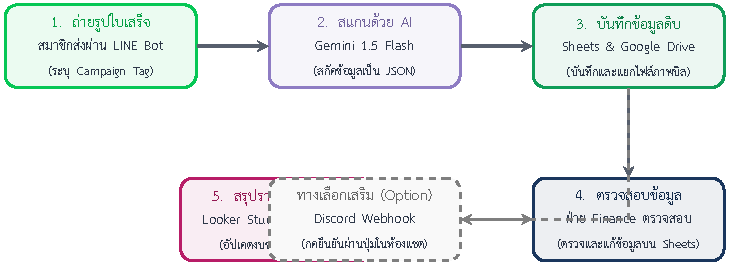
\includegraphics[width=0.85\textwidth]{diagram_finance.png}
  \caption{\chulafont สถาปัตยกรรมกระบวนการตรวจสอบเอกสารและเบิกจ่ายเงินของระบบ ClearBook}
\end{figure}
\vskip 0.2cm

\subsection{โครงสร้างชุดข้อมูลการเบิกจ่าย (Finance Data Schema)}
\begin{table}[h!]
  \centering
  \caption{\chulafont ตัวอย่างคลังข้อมูลรายการเบิกจ่ายของระบบ ClearBook}
  \begin{tabular}{lllrccl}
    \toprule
    \textbf{TX ID} & \textbf{Submitter} & \textbf{Dept} & \textbf{Amount} & \textbf{Store Name} & \textbf{Status} & \textbf{Campaign Tag} \\
    \midrule
    TX-2601 & Four & Innovation & 450.00 & Cafe Amazon & Approved & Recruiter-2026 \\
    TX-2602 & Peach & Marketing & 1,500.00 & Meta Ads & Approved & Recruiter-2026 \\
    TX-2603 & Guy & Activity & 3,200.00 & Somtum Shop & Pending & Workshop-AI \\
    TX-2604 & View & Marketing & 900.00 & Canva Pro & Approved & Startup-Idea \\
    \bottomrule
  \end{tabular}
\end{table}

\subsection{เครื่องมือที่เลือกใช้และเหตุผลเชิงเทคนิค}
\begin{itemize}
  \item \textbf{LINE Messaging API}: เป็นแอปพลิเคชันหลักที่นิสิตทุกคนใช้งานประจำวัน ทำให้อัตราการใช้งานระบบของสมาชิก (Adoption Rate) มีระดับสูงโดยไม่ต้องเสียแรงผลักดัน
  \item \textbf{Gemini 1.5 Flash API}: มีขีดความสามารถสกัดข้อมูลจากเอกสารภาษีทั้งภาษาไทยและภาษาอังกฤษได้แม่นยำ และยังมีความเสถียรในการคืนค่าโครงสร้างข้อมูลเป็น JSON ตามกำหนดได้อย่างมั่นคง
  \item \textbf{Discord / LINE Webhook}: ช่วยกระตุ้นกระบวนการกดยืนยัน (Approve) โดยดึงข้อมูลและปุ่มดำเนินการส่งตรงให้ผู้รับผิดชอบทำต่อได้ทันที
\end{itemize}

\subsection{การต่อยอดความสามารถในอนาคต (Future Extensions)}
ระบบสามารถขยายขีดความสามารถการแจ้งเตือนและการป้องกันความเสี่ยง เช่น ระบบคัดกรองใบเสร็จซ้ำซ้อนหรือตรวจจับความผิดปกติ (Anomaly and Fraud Detection) โดยแจ้งเตือนในทันทีหากตรวจพบใบเสร็จที่มี วันที่ เวลา ร้านค้า และยอดเงินซ้ำกันในระบบฐานข้อมูลเพื่อป้องกันการส่งเบิกเงินซ้ำสองครั้ง

\subsection{ตัวชี้วัดความสำเร็จของระบบ (Success Metrics)}
\begin{itemize}
  \item \textbf{เวลาเบิกจ่ายที่ประหยัดได้}: นิสิตพิมพ์กรอกข้อมูลลดลงกว่า 90\% และระยะเวลาดำเนินการอนุมัติลดลงเหลือไม่ถึง 10 นาที
  \item \textbf{ความสูญเสียเอกสาร}: อัตราการสูญหายหรือการลิงก์ภาพหมดอายุลดลงจนเป็น 0\% ด้วยระบบ Cloud Auto-archive
  \item \textbf{ความโปร่งใสทางการคลัง}: ฝ่ายบริหารเห็นตัวเลขงบประมาณคงเหลือจริงแบบ Real-time 24 ชั่วโมงต่อวัน
\end{itemize}

\newpage

\section{บูรณาการเชิงระบบ: การวิเคราะห์ความคุ้มค่าแคมเปญการตลาดข้ามแผนก (Campaign ROI)}
\subsection{แนวคิดเชิงระบบและความคุ้มค่าแบบบูรณาการ}
จุดปิดเกมสำคัญของการออกแบบ **Club OS** คือความสามารถในการผสานข้อมูลข้ามกระทรวง (Cross-department Integration) เพื่อการตัดสินใจที่มีคุณภาพสูงสุด 

\begin{highlightbox}
  \noindent \textbf{The Synergy Loop:} 
  ข้อมูลค่าใช้จ่ายทางการตลาด เช่น ค่าเช่าสถานที่ ค่าพิมพ์ใบปลิวประชาสัมพันธ์ หรือค่ายิงโฆษณาในเพจเฟซบุ๊กจะถูกบันทึกผ่านทางโมดูล **ClearBook** และทำเครื่องหมายเพื่อเชื่อมโยงธุรกรรมด้วยรหัสเดียวกันคือ **Campaign Tag** ในขณะเดียวกันสถิติที่ได้จากการปล่อยประชาสัมพันธ์หรือคอนเทนต์โปรโมตแคมเปญนั้นจะถูกจัดเก็บในโมดูล **Social Pulse** โดยอ้างอิงผ่าน **Campaign Tag** เดียวกัน 

  เมื่อระบบหลังบ้านทำการเชื่อมต่อและจับคู่ฐานข้อมูลทั้งสองตารางตามรหัส Campaign Tag เดียวกัน ระบบจะช่วยให้ฝ่ายบริหารเห็นประสิทธิภาพในการจัดสรรงบประมาณที่แท้จริงตามสูตรคำนวณด้านล่างนี้
\end{highlightbox}

\begin{equation}
  \text{Cost per Reach (CPR)} = \frac{\text{ยอดเงินใช้จ่ายรวมในโครงการ (จาก ClearBook)}}{\text{ยอดจำนวนการเข้าถึงรวม (จาก Social Pulse)}}
\end{equation}

\begin{equation}
  \text{Cost per Engagement (CPE)} = \frac{\text{ยอดเงินใช้จ่ายรวมในโครงการ (จาก ClearBook)}}{\text{ยอดจำนวนการมีส่วนร่วมรวม (จาก Social Pulse)}}
\end{equation}

\vskip 0.2cm
\begin{figure}[h!]
  \centering
  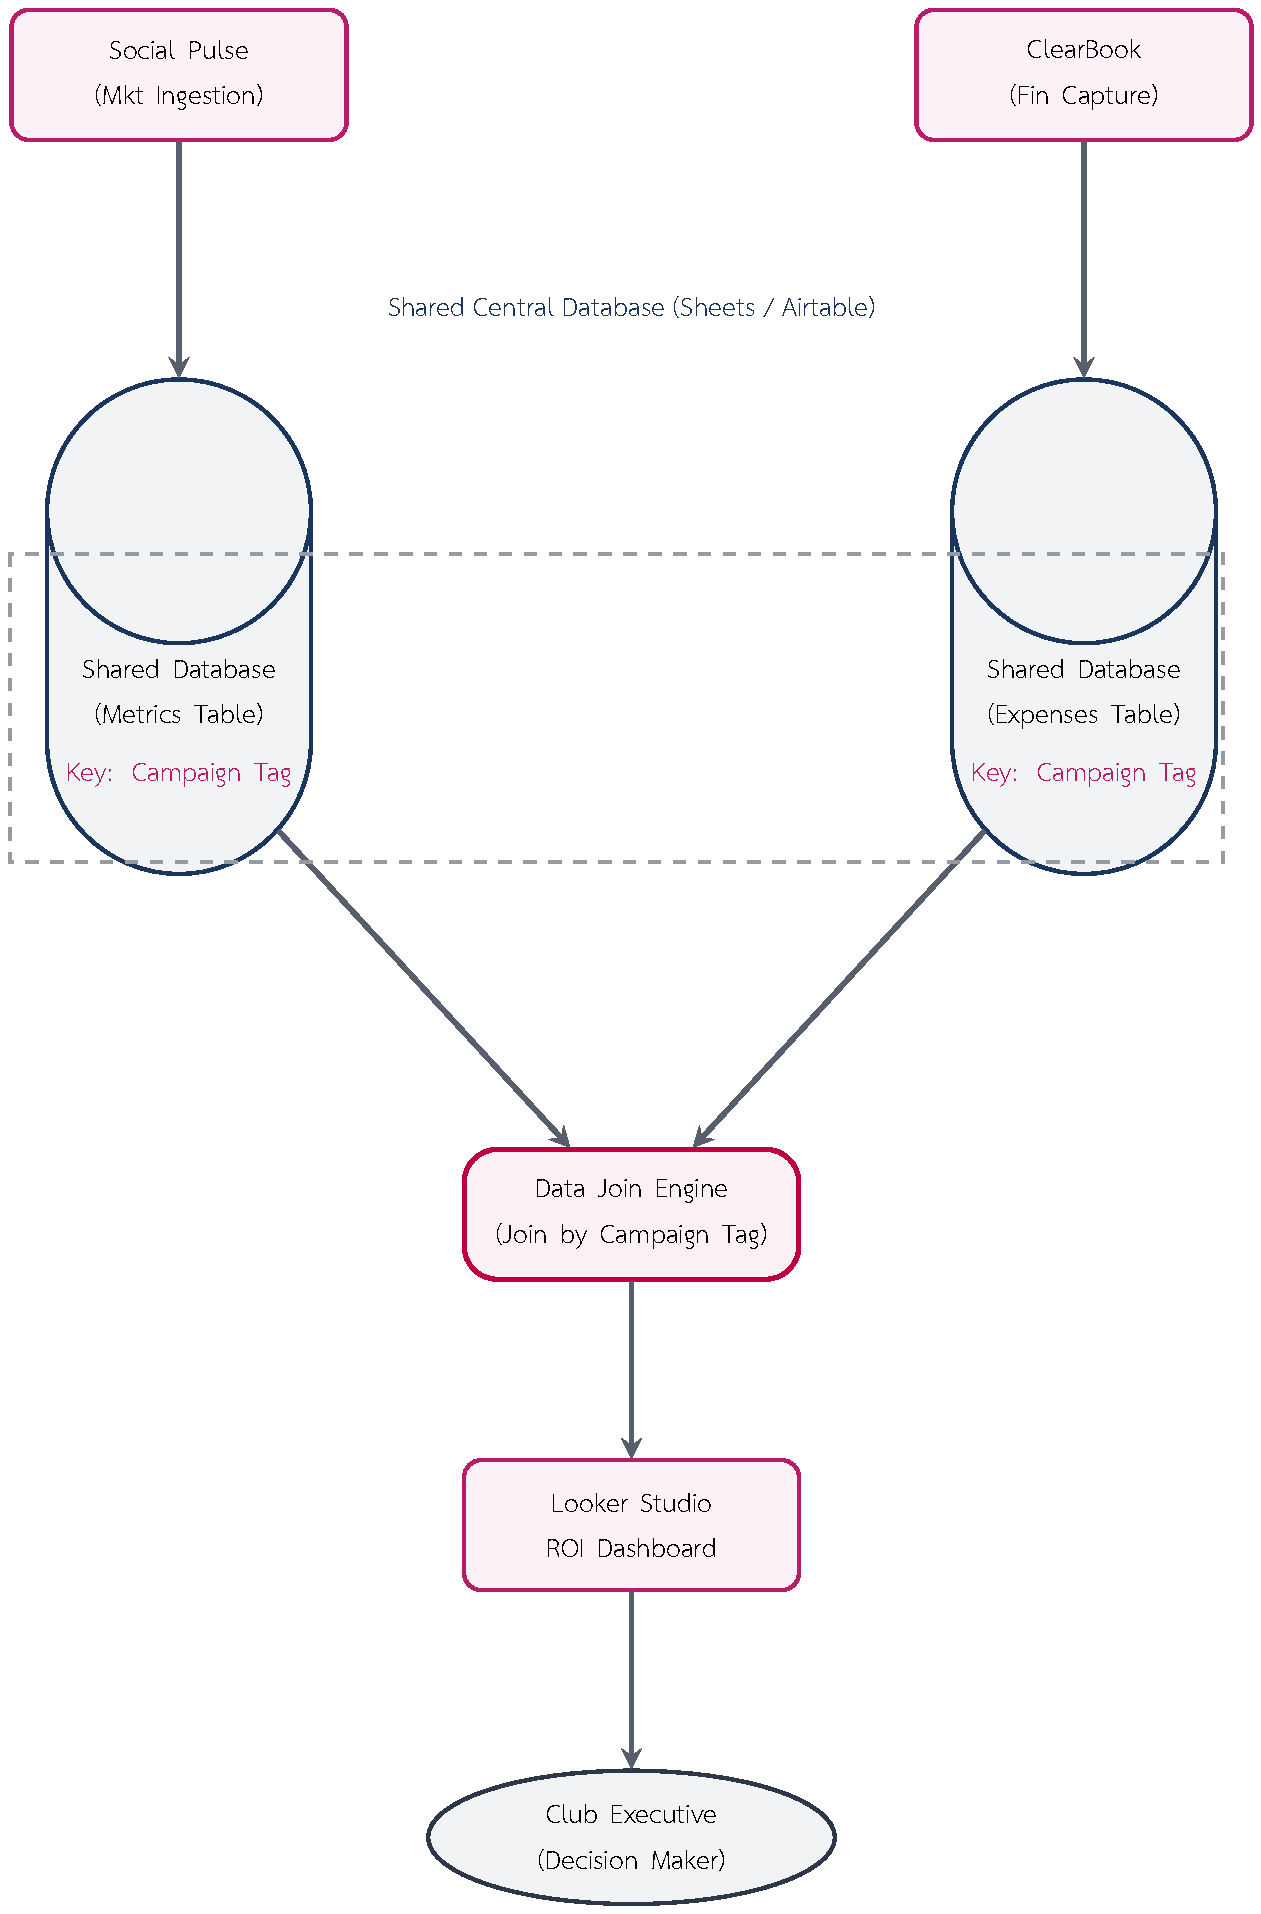
\includegraphics[width=0.9\textwidth]{diagram_club_os.png}
  \caption{\chulafont แผนภาพการเชื่อมโยงระบบข้อมูลข้ามแผนกเพื่อประเมินผลสัมฤทธิ์ทางการเงินและการตลาดร่วมกัน}
\end{figure}
\vskip 0.2cm

\subsection{ประโยชน์สูงสุดต่อการตัดสินใจระดับบริหาร}
แดชบอร์ดสรุปยอดตัวชี้วัด CPR และ CPE ช่วยตอบคำถามสำคัญให้แก่คณะกรรมการและประธานชมรมได้ เช่น:
\begin{itemize}
  \item แคมเปญประชาสัมพันธ์การรับสมัครสมาชิกใหม่ประจำปี (Recruiter-2026) ใช้งบประมาณยิงโฆษณา 2,400 บาท (บันทึกโดย ClearBook) สามารถช่วยขยายยอดการเข้าถึงหน้าเพจรวม 18,200 ครั้ง และสร้างยอดการมีส่วนร่วม 3,630 ครั้ง (บันทึกโดย Social Pulse) คิดเป็นต้นทุนที่ \textbf{0.13 บาทต่อ Reach} และ \textbf{0.66 บาทต่อ Engagement}
  \item เมื่อเปรียบเทียบกับ แคมเปญการจัดเวิร์กชอปความรู้ (Workshop-AI) ที่ใช้งบประมาณ 3,200 บาท แต่ได้ยอดผู้เห็นคอนเทนต์ต่ำเนื่องจากโพสต์ภาพนิ่งเฉยๆ ทำให้มีค่าโฆษณาที่สูงเกินความเหมาะสม ฝ่ายบริหารสามารถนำชุดข้อมูลนี้ไปตัดสินใจในการเลือกเทงบประมาณให้คอนเทนต์วิดีโอในกิจกรรมครั้งถัดไปได้ทันที
\end{itemize}

\newpage

\section{แผนการดำเนินงานและการทดสอบระบบ (Phased Rollout \& Success Metrics)}
ฝ่าย Innovation กำหนดแผนการดำเนินงานพัฒนาระบบแบ่งออกเป็น 3 ระยะเพื่อให้มั่นใจว่าระบบจะมีความพร้อมในการทดสอบและเกิดผลกระทบที่แท้จริงอย่างรวดเร็วภายใต้งบประมาณการใช้งานในระดับศูนย์

\subsection{แผนการดำเนินงานแบ่งออกเป็น 3 ระยะ}
\begin{enumerate}[label=\bfseries ระยะที่ \arabic*:]
  \item \textbf{ระยะเริ่มต้น (Weeks 1-2) - Minimum Viable Product (MVP)}:
  เริ่มพัฒนาระบบดึงภาพใบเสร็จเข้าห้องแชตและใช้ Gemini 1.5 Flash API ทำการ OCR ส่งสแกนบันทึกลง Google Sheets และส่งลิงก์ภาพเก็บเข้าสู่ระบบจัดเก็บไฟล์ Google Drive เป็นการแก้ไขปัญหาเอกสารทางการเงินหลักสูญหายได้ทันที ในขณะที่ฝ่าย Marketing จะเริ่มทดสอบใช้งานช่องทางกรอกข้อมูลแบบด่วนผ่านแบบฟอร์มกูเกิลฟอร์มเป็นหลักเพื่อรวบรวมโครงสร้างชุดข้อมูลการตลาด
  
  \item \textbf{ระยะเสถียรและระบบอัตโนมัติ (Weeks 3-4) - Full Automation}:
  ทำการต่อยอดโดยเขียนท่อข้อมูลดึงสถิติคอนเทนต์ผ่านทาง Meta/TikTok API บน Make.com เพื่อเชื่อมข้อมูลแบบเรียลไทม์ และทำการติดตั้งระบบทบทวนข้อมูลใบเสร็จผ่านปุ่มกดยืนยันธุรกรรม (Approve Button) ในกลุ่มบอท LINE และ Discord ของคณะกรรมการฝ่ายคลัง
  
  \item \textbf{ระยะเชื่อมโยงผลตอบแทน (Week 5) - Shared Analytics}:
  ปรับปรุงแดชบอร์ดในระบบ Looker Studio ให้สามารถดึงฐานข้อมูลทั้งสองระบบมาสรุปวิเคราะห์ร่วมกันผ่านฟิลด์เชื่อมต่อ Campaign Tag เพื่อสร้างข้อวิเคราะห์ผลตอบแทนทางการเงินและกลยุทธ์การตลาด (Campaign ROI) ส่งต่อแก่ฝ่ายประธาน
\end{enumerate}

\subsection{ตารางสรุปเปรียบเทียบผลลัพธ์ประสิทธิภาพก่อนและหลังการพัฒนาติดตั้งระบบ}
\begin{table}[h!]
  \centering
  \caption{\chulafont ตารางเปรียบเทียบสถิติเชิงการดำเนินงานก่อนและหลังปรับปรุงระบบของชมรม}
  \begin{tabular}{lll}
    \toprule
    \textbf{ตัวชี้วัดที่ทำการประเมิน} & \textbf{กระบวนการทำงานแบบเดิม (Manual)} & \textbf{ระบบใหม่แบบอัตโนมัติ (Club OS)} \\
    \midrule
    \textbf{เวลาที่ใช้เก็บสถิติ Marketing} & 3-4 ชั่วโมง ต่อสัปดาห์ (พิมพ์มือ) & 0 นาที (ระบบดึงสถิติให้อัตโนมัติเวลาเที่ยงคืน) \\
    \textbf{เวลาเฉลี่ยบันทึกและตรวจสอบใบเสร็จ} & 3-5 วันทำการ (ต้องทวงเอกสารย้อนหลัง) & ภายใน 5-10 นาที (นิสิตส่งใบเบิกทันทีที่จ่ายเงิน) \\
    \textbf{ความถูกต้องของหลักฐานการเบิกจ่าย} & ปานกลาง (รูปในแชตมักมีลิงก์หมดอายุ) & 100\% (จัดเก็บถาวรและสกัดยอดเงินด้วย AI) \\
    \textbf{งบประมาณซอฟต์แวร์รายปีของชมรม} & 0 บาท (ใช้นิสิตทำงานซ้ำซาก) & 0 บาท (ใช้งานเทคโนโลยี Serverless และ Free Tier) \\
    \textbf{การเข้าถึงข้อมูลเพื่อตัดสินใจกลยุทธ์} & ไม่มีระบบการเปรียบเทียบ ROI & แสดงผล CPR และ CPE บน Looker Studio เรียลไทม์ \\
    \bottomrule
  \end{tabular}
\end{table}

\subsection{บทวิเคราะห์เชิงระบบ (Systems Thinking Insight)}
สถาปัตยกรรมระบบ **Club OS** ช่วยเปลี่ยนบทบาทหน้าที่ของฝ่ายเทคโนโลยีและนวัตกรรม (Innovation Team) จากเดิมที่เป็นฝ่ายคอยเขียนโค้ดและแก้ไขปัญหาไอทีทั่วไป ให้เป็นศูนย์กลางเชิงยุทธศาสตร์ที่ขับเคลื่อนชมรมด้วยโครงสร้างพื้นฐานด้านข้อมูล 

การเชื่อมโยงระบบกระตุ้นกระบวนการทำงานให้เป็นรอบฟีดแบ็กที่มีความเร็วสูง (Fast Feedback Loop) ปลดล็อกความสามารถของฝ่ายการตลาดในการวิเคราะห์เทรนด์ความต้องการของนิสิตข้ามแพลตฟอร์มรายวัน ในขณะที่ช่วยลดความยุ่งยากในการลงบัญชีรายวันของแผนกการเงินให้กลายเป็นเรื่องที่สะดวก รวดเร็ว โปร่งใส และเปิดโอกาสให้นิสิตแกนนำผู้ก่อตั้งชมรมทุกคนสามารถใช้จ่ายทุนโครงการเพื่อสร้างการเติบโตและการมีส่วนร่วมของนิสิตจุฬาลงกรณ์มหาวิทยาลัยได้อย่างคุ้มค่าที่สุด

\end{document}
